\documentclass[12pt]{article}
\usepackage[utf8]{inputenc}
\usepackage[frenchb]{babel}
\RequirePackage[usenames,dvipsnames,xcolor=pst]{pstricks}
\RequirePackage{epsfig} % for eps fig
\RequirePackage{pst-blur} % for nice shadow
\RequirePackage{pst-dbicons} % for E/R
%\RequirePackage{mon-pst-uml} % for my own UML package
\RequirePackage{pst-uml} % for my own UML package
\RequirePackage{tikz} % circles such as History pseudostate
\newcommand{\monpsgrid}{\psgrid}
%\newcommand{\monpsgrid}{}
\setlength{\topmargin}{-5mm}%
\setlength{\oddsidemargin}{-1mm}%
\setlength{\evensidemargin}{-1mm}%
\setlength{\textwidth}{15.5cm}%
\setlength{\textheight}{8.9in}%
%------------------------------------      
%   QCM
%------------------------------------      
%\usepackage[french,correction]{qcm} % to print correct answers
%\usepackage[french]{qcm}
\title{\vspace{-3pc}\textbf{Contr\^ole M2105 (S2 -- 	IHM)}}

\date{Vendredi 11 avril 2014 -- Une seule feuille A4 manuscrite autoris\'ee\\
Dur\'ee : 1h00}

\def\dc{\textsf{diagramme de classe}}
\def\sni{\textsf{SNI}}
\def\ds{\textsf{diagramme de s\'equence}}
\def\dss{\textsf{diagramme de s\'equence syst\`eme}}
%===========================================================
\begin{document}
\maketitle

\section{Liens entre diagrammes}

Sur la figure ci-dessous\footnote{Recopiez la figure sur votre copie.} supprimez les liens que vous considérez inutiles, placez des directions sur les liens entre éléments si besoin, et donnez un nom qui fait sens sur les liens que vous laissez. Vous pourrez vous inspirer du lien \textsf{code} - \sni{} déjà présent.

\scalebox{0.6}{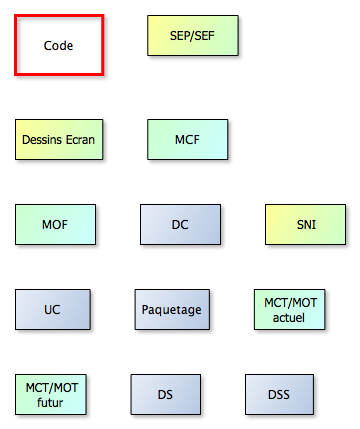
\includegraphics{fig-enchainement-sujet}}

\section{Expertise}

Les services secrets ont intercepté les extraits cryptés d'un \sni{} (a) et de son \dc{} correspondant (b) ci-dessous :

\scalebox{0.6}{\includegraphics{7erreurs}}

Ils vous demandent d'expertiser ces diagrammes pour voir si malgré le cryptage vous pouvez certifier s'ils sont corrects, et si non, proposer une correction.

\section{Ecrire un SNI}

\subsection*{Sujet}

Soit le cahier des charges suivant :

\begin{quote}
On souhaite réaliser le site d'une boutique proposant à la vente des livres et des DVDs. La navigation dans le site devra se faire comme suit :
\begin{itemize}
\item à partir de la page d'accueil, l'internaute peut cliquer sur «\,recherche\,» pour rechercher un produit ou sur
« produits » pour feuilleter le catalogue entier.
\item à partir de la page « recherche », l'internaute fournit un mot pour rechercher un titre de produit. Une liste de résultats est alors présentée. 
S'il clique sur un produit, la page du produit s'affiche.
\item à partir de la page « produit », une liste d'ouvrages est présentée. Si l'internaute clique sur un ouvrage, la page du produit s'affiche.
\end{itemize}
\end{quote}

Un diagramme des cas d'utilisation est donné dans la figure ci-dessous :

\scalebox{0.6}{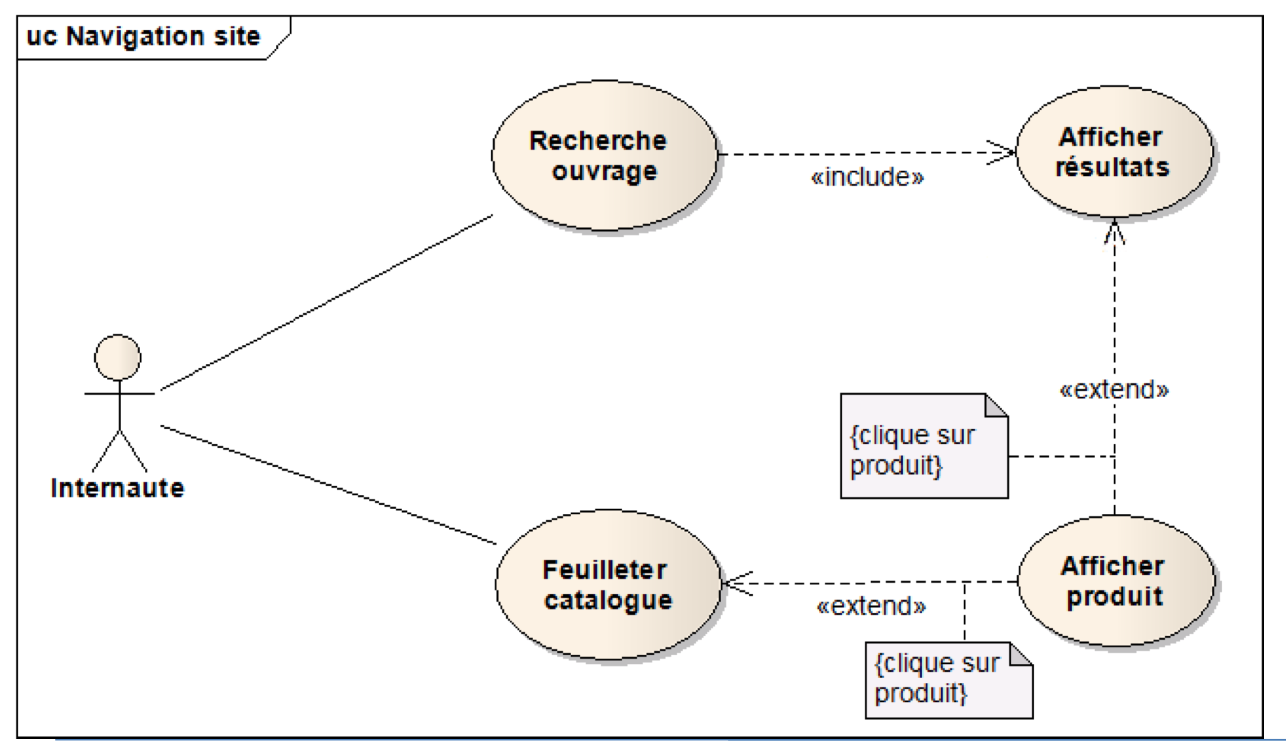
\includegraphics{etude-uc}}

\subsection*{Question}

Réalisez un \sni{} correspondant aux attentes.

\section{Diagramme de classe à partir d'un SNI}

\subsection*{Sujet}

Soit le \sni{} suivant :

\scalebox{0.4}{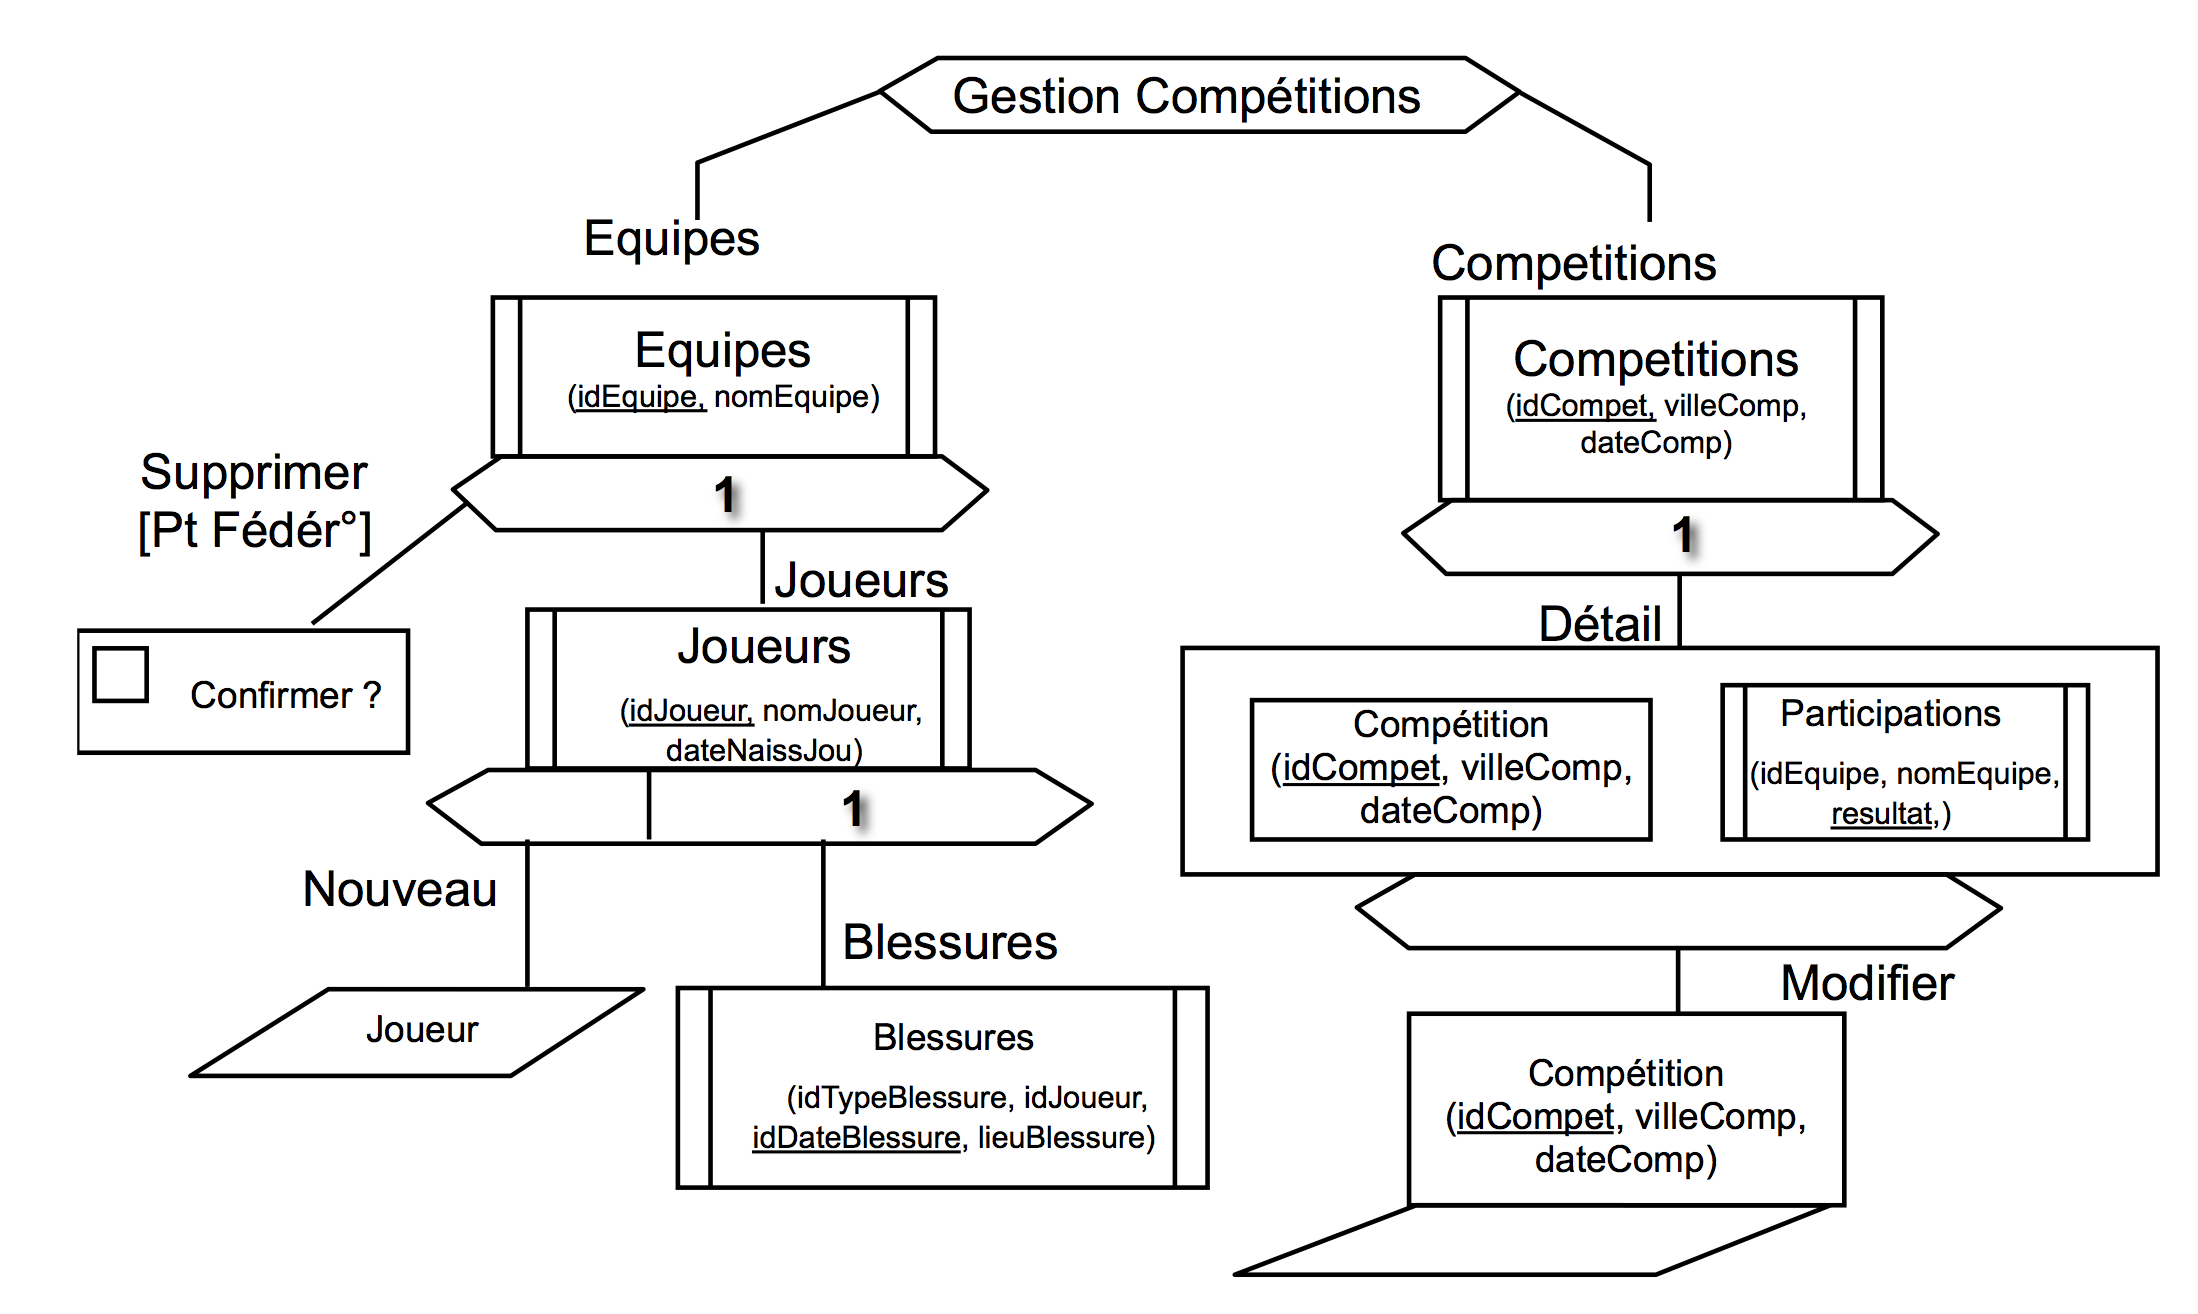
\includegraphics{images/FFF-SNI}}

\subsection*{Question}

Réalisez un \dc{} respectant ce \sni. Celui-ci ne comportera que des éléments déduits du \dc. D'ailleurs vous pourrez numéroter chaque élément de votre diagramme et proposer une légende pour chacun de ces éléments, à la suite de votre diagramme, qui
précise la justification de cet élément.

\section{Mot croisés}

Réalisez le mot croisé fourni en annexe et trouvez le mot mystère en lien avec le module M2105.

\section*{Bar\`eme prévisionnel}

\begin{description}
\item[1] 3 points 
\item[2] 3 points 
\item[3] 4 points 
\item[4] 5 points 
\item[5] 4 points 
\item[Propret\'e]  1 point 
\end{description}

\end{document}
%===========================================================